\documentclass[12pt,a4paper]{article}
\usepackage[polish]{babel}
\usepackage[T1]{fontenc}
\usepackage{lmodern}
\usepackage[utf8x]{inputenc}
\usepackage{hyperref}
\usepackage{url}
\usepackage{graphicx}
\usepackage{listings}
\usepackage[dvipsnames]{xcolor}
\usepackage{color}
\usepackage{float}
\usepackage{multicol}
\usepackage{tikz}
\usepackage{makecell}
% LISTINGS
\definecolor{bluekeywords}{rgb}{0,0,1}
\definecolor{greencomments}{rgb}{0,0.5,0}
\definecolor{redstrings}{rgb}{0.64,0.08,0.08}
\definecolor{xmlcomments}{rgb}{0.5,0.5,0.5}
\definecolor{types}{rgb}{0.17,0.57,0.68}
\usepackage{listings}
\lstset{language=[Sharp]C,
captionpos=b,
frame=lines,
showspaces=false,
showtabs=false,
breaklines=true,
showstringspaces=false,
breakatwhitespace=true,
escapeinside={(*@}{@*)},
commentstyle=\color{greencomments},
morekeywords={partial, var, value, get, set},
keywordstyle=\color{bluekeywords},
stringstyle=\color{redstrings},
basicstyle=\ttfamily\footnotesize ,
tabsize=4,
}
\lstdefinelanguage{Kotlin}{
  comment=[l]{//},
  commentstyle={\color{gray}\ttfamily},
  emph={delegate, filter, first, firstOrNull, forEach, lazy, map, mapNotNull, println, return@},
  emphstyle={\color{OrangeRed}},
  identifierstyle=\color{black},
  keywords={abstract, actual, as, as?, break, by, class, companion, continue, data, do, dynamic, else, enum, expect, false, final, for, fun, get, if, import, in, interface, internal, is, null, object, override, package, private, public, return, set, super, suspend, this, throw, true, try, typealias, val, var, vararg, when, where, while},
  keywordstyle={\color{NavyBlue}\bfseries},
  morecomment=[s]{/*}{*/},
  morestring=[b]",
  morestring=[s]{"""*}{*"""},
  ndkeywords={@Deprecated, @JvmField, @JvmName, @JvmOverloads, @JvmStatic, @JvmSynthetic, Array, Byte, Double, Float, Int, Integer, Iterable, Long, Runnable, Short, String},
  ndkeywordstyle={\color{BurntOrange}\bfseries},
  sensitive=true,
  stringstyle={\color{ForestGreen}\ttfamily},
}
% FOREST
\usepackage[edges]{forest}

\definecolor{foldercolor}{RGB}{124,166,198}

\tikzset{pics/folder/.style={code={%
    \node[inner sep=0pt, minimum size=#1](-foldericon){};
    \node[folder style, inner sep=0pt, minimum width=0.3*#1, minimum height=0.6*#1, above right, xshift=0.05*#1] at (-foldericon.west){};
    \node[folder style, inner sep=0pt, minimum size=#1] at (-foldericon.center){};}
    },
    pics/folder/.default={20pt},
    folder style/.style={draw=foldercolor!80!black,top color=foldercolor!40,bottom color=foldercolor}
}

\forestset{is file/.style={edge path'/.expanded={%
        ([xshift=\forestregister{folder indent}]!u.parent anchor) |- (.child anchor)},
        inner sep=1pt},
    this folder size/.style={edge path'/.expanded={%
        ([xshift=\forestregister{folder indent}]!u.parent anchor) |- (.child anchor) pic[solid]{folder=#1}}, inner ysep=0.6*#1},
    folder tree indent/.style={before computing xy={l=#1}},
    folder icons/.style={folder, this folder size=#1, folder tree indent=3*#1},
    folder icons/.default={12pt},
}

% SETTINGS
\addtolength{\hoffset}{-1.5cm}
\addtolength{\marginparwidth}{-1.5cm}
\addtolength{\textwidth}{3cm}
\addtolength{\voffset}{-1cm}
\addtolength{\textheight}{2.5cm}
\setlength{\topmargin}{0cm}
\setlength{\headheight}{0cm}
\renewcommand{\arraystretch}{1.5}

% JSON 
\colorlet{punct}{red!60!black}
\definecolor{background}{HTML}{EEEEEE}
\definecolor{delim}{RGB}{20,105,176}
\colorlet{numb}{magenta!60!black}
\lstdefinelanguage{json}{
    basicstyle=\normalfont\ttfamily,
   % numbers=left,
    numberstyle=\scriptsize,
    stepnumber=1,
    numbersep=8pt,
    showstringspaces=false,
    breaklines=true,
    frame=lines,
    backgroundcolor=\color{background},
    literate=
     *{0}{{{\color{numb}0}}}{1}
      {1}{{{\color{numb}1}}}{1}
      {2}{{{\color{numb}2}}}{1}
      {3}{{{\color{numb}3}}}{1}
      {4}{{{\color{numb}4}}}{1}
      {5}{{{\color{numb}5}}}{1}
      {6}{{{\color{numb}6}}}{1}
      {7}{{{\color{numb}7}}}{1}
      {8}{{{\color{numb}8}}}{1}
      {9}{{{\color{numb}9}}}{1}
      {:}{{{\color{punct}{:}}}}{1}
      {,}{{{\color{punct}{,}}}}{1}
      {\{}{{{\color{delim}{\{}}}}{1}
      {\}}{{{\color{delim}{\}}}}}{1}
      {[}{{{\color{delim}{[}}}}{1}
      {]}{{{\color{delim}{]}}}}{1},
}

\title{Type Racer\\Aplikacje mobilne dla systemu Android}
\author{Artur Bednarczyk, Dominika Jurczyk, Damian Fikier\\Politechnika Śląska\\Wydział Matematyki Stosowanej\\Informatyka, semestr V}
\date{\today}

\begin{document}
	\maketitle
	\begin{figure}[H]
		\centering
		
\includegraphics[width=0.5\linewidth]{logo2}
		\label{fig:logo}
	\end{figure}
	\clearpage
	\tableofcontents
	\clearpage
	\section{Zespół}
	\begin{itemize}
	    \item Bednarczyk Artur \begin{itemize}
	        \item Projekt aplikacji - UI i funkcjonalności
	        \item Serwer z Node.js
	        \item Struktura aplikacji - MVP
	        \item Fragmenty i zarządzanie nimi
	        \item RecyclerViewAdapter dla listy wyników
	        \item Model danych
	        \item ''Dialog'' do przesyłania wyniku
	        \item Dokumentacja
	    \end{itemize}
	    \item Jurczyk Dominika \begin{itemize}
	        \item 
	    \end{itemize}
	    \item Fikier Damian \begin{itemize}
	        \item 
	    \end{itemize}
	\end{itemize}
	\clearpage
	\section{Opis projektu}
		\subsection{Opis}
			Gra „Type-Racer”, która polega na wpisywaniu słów pojawiających się na ekranie. Aby słowo zostało zaliczone, musi być wpisane w pełni poprawnie. Po zaliczeniu słowa gracz otrzymuje punkt i pojawia się kolejne słowo. Rozgrywka trwa określony czas. Po zakończeniu gracz ma możliwość przesłania swojego wyniku na serwer, gdzie jest przechowywana lista najlepszych wyników, którą będzie można zobaczyć w aplikacji. Aplikacja będzie posiadała również instrukcję i opis.

		\subsection{Projekt UI}
			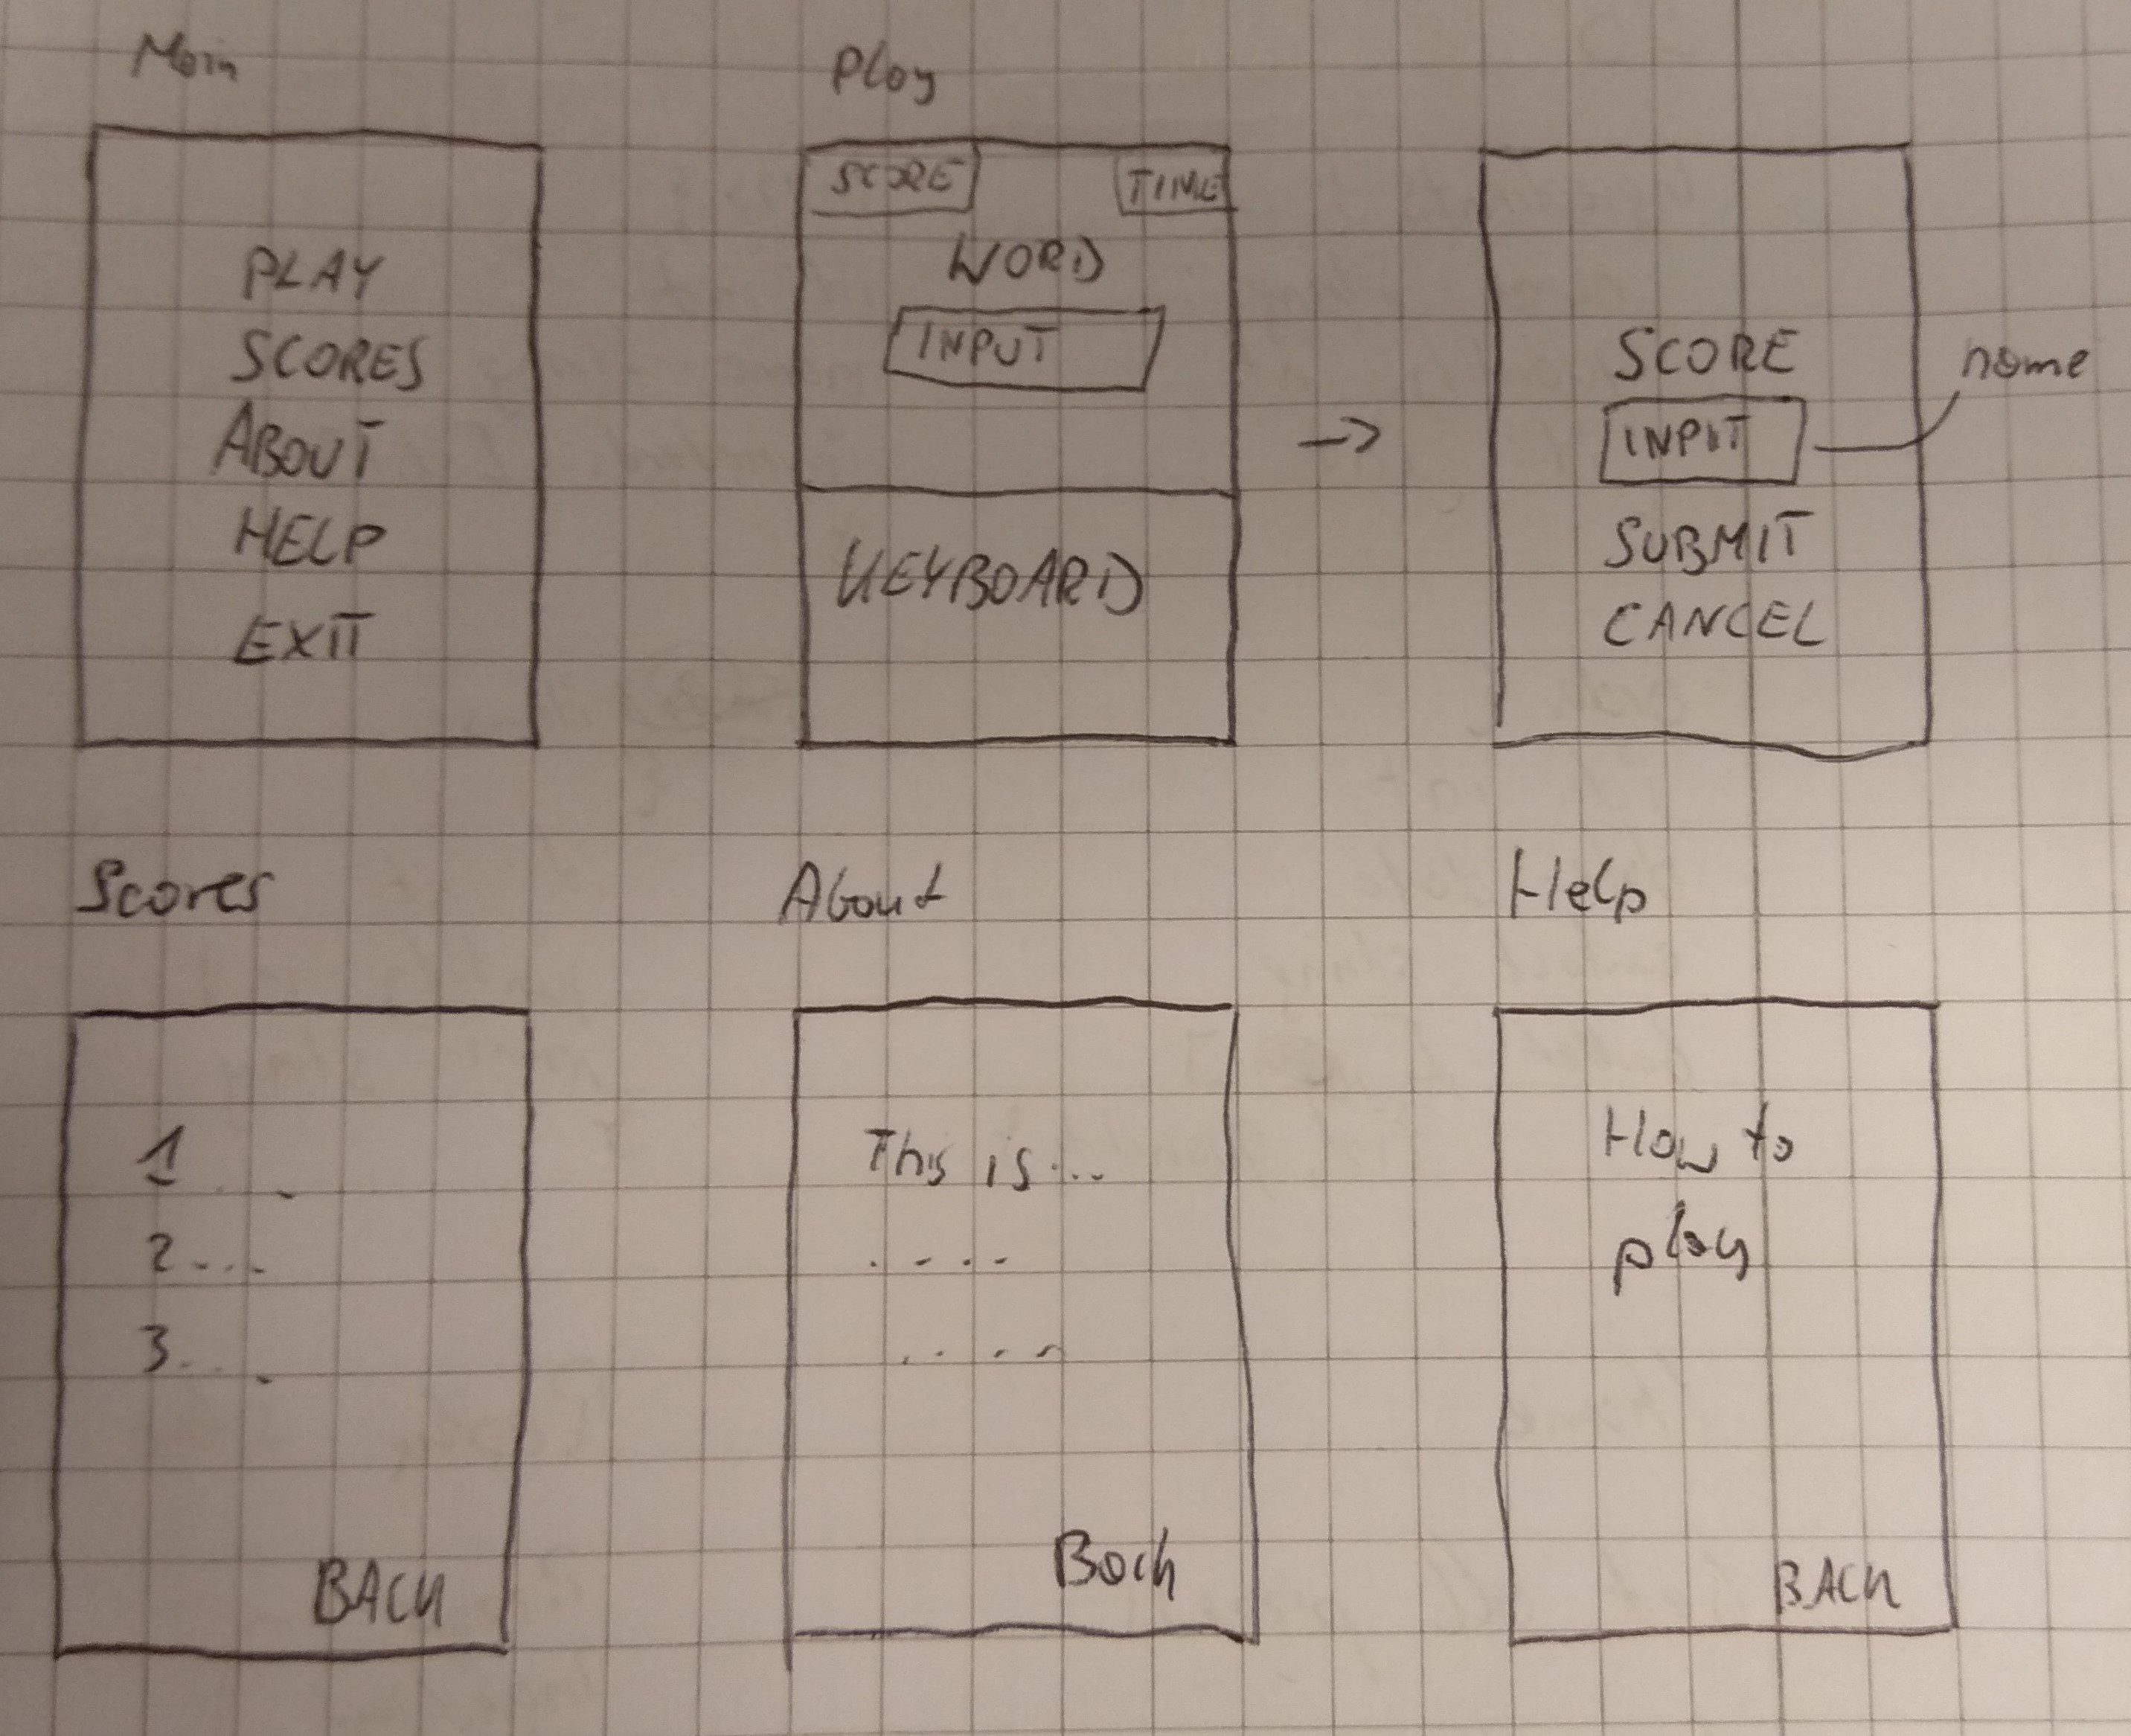
\includegraphics[width=\textwidth]{uiProject.jpg}
			
\clearpage	\subsection{Funkcjonalności}
			\subsubsection{Gra}
			Wpisywanie jak najszybciej wyświetlonego słowa, poprawne wpisanie słowa gwarantuje punkt oraz wyświetlenie kolejnego słowa. Im więcej słów zostanie wpisanych poprawnie, tym więcej punktów uzyska gracz.
			\subsubsection{Lista wyników}
			Gracz ma możliwość zobaczenia listy najlepszych przesłanych wyników.
			\subsubsection{Zgłaszanie własnego wyniku}
			Po zakończeniu rozgrywki gracz może przesłać swój wynik na serwer.
			\subsubsection{Instrukcja i opis}
			Gra zawiera instrukcję oraz opis.
	\section{Technologie, narzędzia}
			\begin{itemize}
			\item Android Studio - Środowisko programistyczne.
			\item GitHub - Repozytorium do przechowywania wersji online.
			\item Heroku - platforma, która przechowuje nasz serwer w chmurze.
			\item mLab - baza danych na listę wyników
			\item Kotlin - aplikacja na platformę Android
			\item MongoDB - baza danych
			\item Node.js - serwer
			\end{itemize}
			\clearpage
	\section{Implementacja}
		\subsection{Podział projektu na pliki}
		\begin{multicols}{2}
\scalebox{0.9}[0.8]{
			\begin{forest}
				for tree={font=\sffamily, grow'=0,
    folder indent=.3em, folder icons}
    	[Main
    	    [.Model
    	        [.DataModels
    	        [MockData.kt, is file]
    	        [ScoreList.kt, is file]
    	        ]
    	        [.Interface
    	        [IAPI.kt, is file]
    	        [IGameInteractor.kt, is file]
    	        [IScore.kt, is file]
    	        [IScoreInteractor.kt, is file]
    	        [IScoreList.kt, is file]
    	        ]
    	        [.Repository
    	        [API.kt, is file]
    	        [MockAPI.kt, is file]
    	        ]
    	        [GameInteractor.kt, is file]
    	        [ScoreInteractor.kt, is file]
    	    ]
    	    [.Presenters
    	    [GamePresenter.kt, is file][ScorePresenter.kt, is file]]
    	    [.Views
    	    [.Fragments
    	    [AboutFragment.kt, is file]
    	    [GameFragment.kt, is file]
    	    [HelpFragment.kt, is file]
    	    [MenuFragment.kt, is file]
    	    [ScoreFragment.kt, is file]
    	    [ScoreRecuclerViewAdapter.kt, is file]
    	    ]
    	    [.Interface [IGameBoard.kt, is file][IMainActivity.kt, is file][IScoreBoard.kt, is file]]
    	    [MainActivity.kt, is file]
    	    [VIEWS.kt, is file]
    	    ]
    	]
			\end{forest}
			}
\scalebox{0.9}[0.8]{
			\begin{forest}
				for tree={font=\sffamily, grow'=0,
                folder indent=.3em, folder icons}
    [res
        [.layout 
            [activity\_main.xml, is file]
            [custom\_dialog.xml, is file]
            [fragment\_about.xml, is file]
            [fragment\_game.xml, is file]
            [fragment\_help.xml, is file]
            [fragment\_menu.xml, is file]
            [fragment\_score.xml, is file]
            [fragment\_score\_list.xml, is file]
        ]
        [.menu 
            [menu.xml, is file]
        ]
        [.values
            [colors.xml, is file]
            [dimens.xml, is file]
            [strings.xml, is file]
            [styles.xml, is file]
        ]
    ]
    \end{forest}
}
		\end{multicols}
\clearpage 
\subsection{Architektura}
%\begin{lstlisting}[caption={Simple code listing.}, label={lst:example1}, language=Kotlin]
%// this is a simple code listing:
%println("hello kotlin from latex")
%\end{lstlisting}
Aplikacja składa się z jednej aktywności, która zawiera fragmenty. Dzięki implementacji odpowiedniego interfejsu, fragmenty mogą komunikować się z aktywnością, co jest wykorzystywane do przełączania się między fragmentami. Fragment z głównym menu, po kliknięciu odpowiedniego przycisku wysyła informację o tym do aktwyności, która podmieni fragment.\\
\begin{lstlisting}[caption={Interfejs oraz wywołanie akcji w fragmencie}, label={lst:example1}, language=Kotlin]
// MenuFragment.kt
private var listenerMenu: OnMenuFragmentInteractionListener? = null
    override fun onCreateView(
        inflater: LayoutInflater, container: ViewGroup?,
        savedInstanceState: Bundle?
    ): View? {
        val view = inflater.inflate(R.layout.fragment_menu, container, false)
        view.playButton.setOnClickListener {
            listenerMenu?.onMenuFragmentInteraction(VIEWS.GAME)
        }
    }
    interface OnMenuFragmentInteractionListener {
        fun onMenuFragmentInteraction(s: VIEWS)
    }
\end{lstlisting}\\
\begin{lstlisting}[caption={Implementacja w aktywności}, label={lst:example2}, language=Kotlin]
// MainActivity.kt
    override fun onMenuFragmentInteraction(s: VIEWS) {
        when (s) {
            VIEWS.MENU -> changeFragment(menuFragment)
            VIEWS.GAME -> changeFragment(gameFragment)
            VIEWS.SCORE -> changeFragment(scoreFragment)
            VIEWS.HELP -> changeFragment(helpFragment)
            VIEWS.ABOUT -> changeFragment(aboutFragment)
            VIEWS.EXIT -> exitGame()
        }
    }
\end{lstlisting}\\
Zastosowany wzorzec Model-View-Presenter pozwolił na oddzielenie logiki od widoku. Aby połączenie było cały czas aktywne ustanawiamy je w metodzie onCreateView danego fragmentu. Konstruktor prezentera wymaga również modelu jaki chcemy stosować. Przykład:\\
\begin{lstlisting}[caption={Połączenie fragmentu z prezenterem}, label={lst:example3}, language=Kotlin]
\\ GameFragment.kt
lateinit var presenter: GamePresenter
    override fun onCreateView(
        inflater: LayoutInflater, container: ViewGroup?,
        savedInstanceState: Bundle?
    ): View? {
        val view = inflater.inflate(R.layout.fragment_game, container, false)
        presenter = GamePresenter(this, GameInteractor())
        presenter.getWord()
        return view
    }
\end{lstlisting}\\
Przykładowa implementacje prezentera:\\
\begin{lstlisting}[caption={Prezenter}, label={lst:example4}, language=Kotlin]
// GamePresenter.kt
class GamePresenter(val view: IGameBoard, val interactor: IGameInteractor){
    fun getWord() {
        view.wordInput.text = interactor.getWord()
    }
}
\end{lstlisting}\\
Prezenter komunikując się z modelem, korzysta z ''Interactor'', który odpowiada za interakcje z danymi.\\
\begin{lstlisting}[caption={Interactor}, label={lst:example5}, language=Kotlin]
// GameInteractor.kt
class GameInteractor : IGameInteractor {
    val API = MockAPI
    override fun getWord(): String {
        return API.getWord()
    }
}
\end{lstlisting}\\
Dane wykorzystywane w aplikacji pobierane są z serwera za pomocą ''Repository'', które zawiera metody odpowiedzialne za wykonywanie zapytań do zewnętrznego serwera. W ramach testowania utworzono fałszywe API\\
\begin{lstlisting}[caption={Repository}, label={lst:example6}, language=Kotlin]
// MockAPI.kt
object MockAPI: IAPI {
    override fun getWord(): String {
        return "randomWORDtest"
    }
}
\end{lstlisting}\\
Model danych: \\
\begin{lstlisting}[caption={Model Danych}, label={lst:example7}, language=Kotlin]
// ScoreList.kt
class ScoreList:IScoreList {
    override val SCORES: MutableList<Score> = ArrayList()

    override fun addScore(score: Score){
        SCORES.add(score)
    }

    data class Score(override val score: Int, override val nick: String) : IScore
}
\end{lstlisting}

\subsection{Schemat Modelu Obiektowego}
			\begin{figure}[H]
			\centering
			\includegraphics[width=1.0\textwidth]{class_diagram}
			\caption{Tu będzie schemat}
			\end{figure}
\subsection{API}
Adres serwera: http://simple-type-racer.herokuapp.com/
\begin{itemize}
    \item 1 słowo
    \begin{itemize}
        \item URL: /server/getWord
        \item metoda: GET
        \item parametry url: brak
        \item odpowiedz: STRING
    \end{itemize}
    \item 5 słów
    \begin{itemize}
        \item URL: /server/getWord
        \item metoda: GET
        \item parametry url: brak
        \item odpowiedz: tablica 5 elementów typu: STRING
    \end{itemize}
    \item zgłaszanie wyniku
    \begin{itemize}
        \item URL: /server/result
        \item metoda: POST
        \item parametry url: brak
        \item parametry w ciele: nickname=[String] oraz score=[Number]
        \item przykładowe ciało zapytania:
                        \begin{lstlisting}[language=json,firstnumber=1]
{
  "nickname": "name",
  "score": 23
}
\end{lstlisting}
        \item odpowiedz: JSON
        \item przykładowa odpowiedź:
                \begin{lstlisting}[language=json,firstnumber=1]
{
    "success": true,
    "info": {
        "_id": "5c27d0d7dd97760015a5391b",
        "nickname": "Isur",
        "score": 11,
        "__v": 0
    }
}
\end{lstlisting}
    \end{itemize}
    \item top 10
    \begin{itemize}
        \item URL: /server/top10
        \item metoda: GET
        \item parametry url: brak
        \item odpowiedz: JSON
        \item przykładowa odpowiedź:
        \begin{lstlisting}[language=json,firstnumber=1]
[
    {
        "_id": "5c1ff3415b36030015bd61c4",
        "nickname": "User1",
        "score": 38,
        "__v": 0
    },
    {
        "_id": "5c27d0d7dd97760015a5391b",
        "nickname": "User2",
        "score": 11,
        "__v": 0
    },
]
\end{lstlisting}
    \end{itemize}
\end{itemize}
\clearpage
\end{document}